\documentclass[border=0.125cm]{standalone}
\usepackage{tikz}
\usetikzlibrary{positioning}
\begin{document}

\definecolor{input_node}{RGB}{171,171,154}
\definecolor{dense_node}{RGB}{196,225,144}
\definecolor{dropout_node}{RGB}{222,222,222}
\definecolor{output_node}{RGB}{171,154,154}
% New colors
\definecolor{klight_green_400}{RGB}{156, 204, 101}

\tikzset{%
  dense neuron/.style={
    circle,
    draw,
    fill=klight_green_400,
    thick,
    minimum size=1cm
  },
  dropout neuron/.style={
    circle,
    draw,
    fill=dropout_node,
    thick,
    minimum size=1cm
  },
  input neuron/.style={
    circle,
    draw,
    fill=input_node,
    thick,
    minimum size=1cm
  },
  output neuron/.style={
    circle,
    draw,
    fill=output_node,
    thick,
    minimum size=1cm
  },
  neuron missing/.style={
    draw=none, 
    scale=4,
    fill=none,
    text height=0.333cm,
    execute at begin node=\color{black}$\vdots$
  },
}

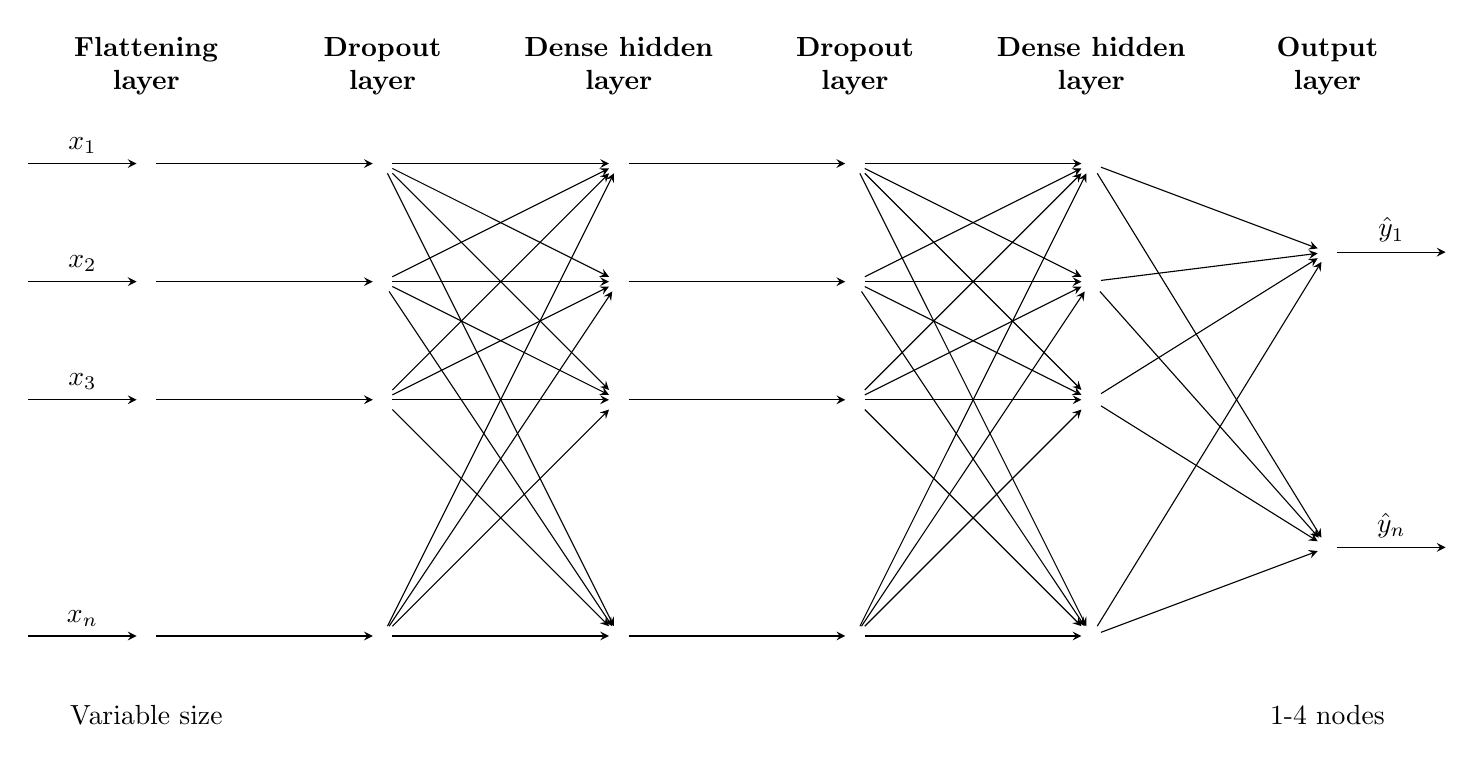
\begin{tikzpicture}[x=1.5cm, y=1.5cm, >=stealth]
% Input layer
\foreach \m/\l [count=\y] in {1,2,3,missing,4}
  \node [input neuron/.try, neuron \m/.try] (input-\m) at (0,2.5-\y) {};
% First dropout layer
\foreach \m/\l [count=\y] in {1,2,3,missing,4}
  \node [dropout neuron/.try, neuron \m/.try] (dropout1-\m) at (2,2.5-\y) {};
% First hidden layer
\foreach \m [count=\y] in {1,2,3,missing,4}
  \node [dense neuron/.try, neuron \m/.try ] (hidden1-\m) at (4,2.5-\y) {};
% Second dropout layer
\foreach \m/\l [count=\y] in {1,2,3,missing,4}
  \node [dropout neuron/.try, neuron \m/.try] (dropout2-\m) at (6,2.5-\y) {};
% Second hidden layer
\foreach \m [count=\y] in {1,2,3,missing,4}
  \node [dense neuron/.try, neuron \m/.try ] (hidden2-\m) at (8,2.5-\y) {};
% Output layer
\foreach \m [count=\y] in {1,missing,2}
  \node [input neuron/.try, neuron \m/.try ] (output-\m) at (10,2-1.25*\y) {};

Draw node labels
\foreach \l [count=\i] in {1,2,3,n}
  \draw [<-] (input-\i) -- ++(-1,0)
    node [above, midway] {$x_\l$};

\foreach \l [count=\i] in {1,n}
  \draw [->] (output-\i) -- ++(1,0)
    node [above, midway] {$\hat{y}_\l$};

% Draw connections
\foreach \i in {1,...,4}
    \draw [->] (input-\i) -- (dropout1-\i);
    
\foreach \i in {1,...,4}
  \foreach \j in {1,...,4}
    \draw [->] (dropout1-\i) -- (hidden1-\j);

\foreach \i in {1,...,4}
    \draw [->] (hidden1-\i) -- (dropout2-\i);
    
\foreach \i in {1,...,4}
  \foreach \j in {1,...,4}
    \draw [->] (dropout2-\i) -- (hidden2-\j);

\foreach \i in {1,2,3,...,4}
  \foreach \j in {1,2}
    \draw [->] (hidden2-\i) -- (output-\j);

\foreach \l [count=\x from 0] in {Flattening, Dropout, Dense hidden, Dropout, Dense hidden, Output}
  \node [align=center, above] at (\x*2,2) {\textbf{\l} \\ \textbf{layer}};
  
\foreach \l [count=\x from 0] in {Variable size, , , , , 1-4 nodes}
  \node [align=center, below] at (\x*2,-3) {\l};

\end{tikzpicture}

\end{document}